\subsection{Hidden Markov Models}

HMMs are common statistical models used to describe time series that exhibit state-switching behaviour. An HMM models an observed sequence of length $T$, $\bfY = \{Y_t\}_{t=1}^T$, together with an unobserved (or  ``hidden") sequence $\bfX = \{X_t\}_{t=1}^T$. The hidden sequence $\bfX$ is a Markov chain, and each observation $Y_t$ is a random variable, where $Y_t$ given all other observations $\bfY \setminus \{Y_t\}$ and hidden states $\bfX$ depends only on $X_t$. While the sample space of $\bfX$ is general, we assume $X_t \in \{1,\ldots,N\}$ for some finite $N$. The unconditional distribution of $X_1$ is denoted by the row-vector $\delta \in \bbR^N$, where $\delta^{(i)} = \bbP(X_1 = i)$. Further, the distribution of $X_t$ for $t > 1$ conditioned on $X_{t-1}$ is denoted by an $N$-by-$N$ transition probability matrix $\Gamma_t$, where $\Gamma_t^{(i,j)} = \bbP(X_t = j \mid X_{t-1} = i)$. %Our methods apply to transition probability matrices that depend upon time, but for ease of presentation
For simplicity, we assume that $\Gamma_t$ does not change over time (i.e. $\Gamma_t = \Gamma$ for all $t$) unless stated otherwise. 

%We assume that the distribution of an observation $Y_t$ conditioned on the corresponding hidden state $X_t$ does not depend upon any other observation or hidden state.
%Some variants of HMMs allow $Y_t$ to depend upon both $Y_{t-1}$ and $X_t$. Our methodology can be straightforwardly applied to such HMMs, but for clarity of presentation we assume that $Y_t$ depends only on $X_t$. 
If $X_t=i$, then we denote the conditional density or probability mass function of $Y_t$ as $f^{(i)}(\cdot ; \theta^{(i)})$ or simply $f^{(i)}$, where $\theta^{(i)}$ is a state-dependent parameter describing the emission distribution. The collection of all state-dependent parameters is $\theta = \{\theta^{(i)}\}_{i=1}^N$. Figure \ref{fig:HMM} shows an HMM as a graphical model.

\begin{figure}[h]
    \centering
    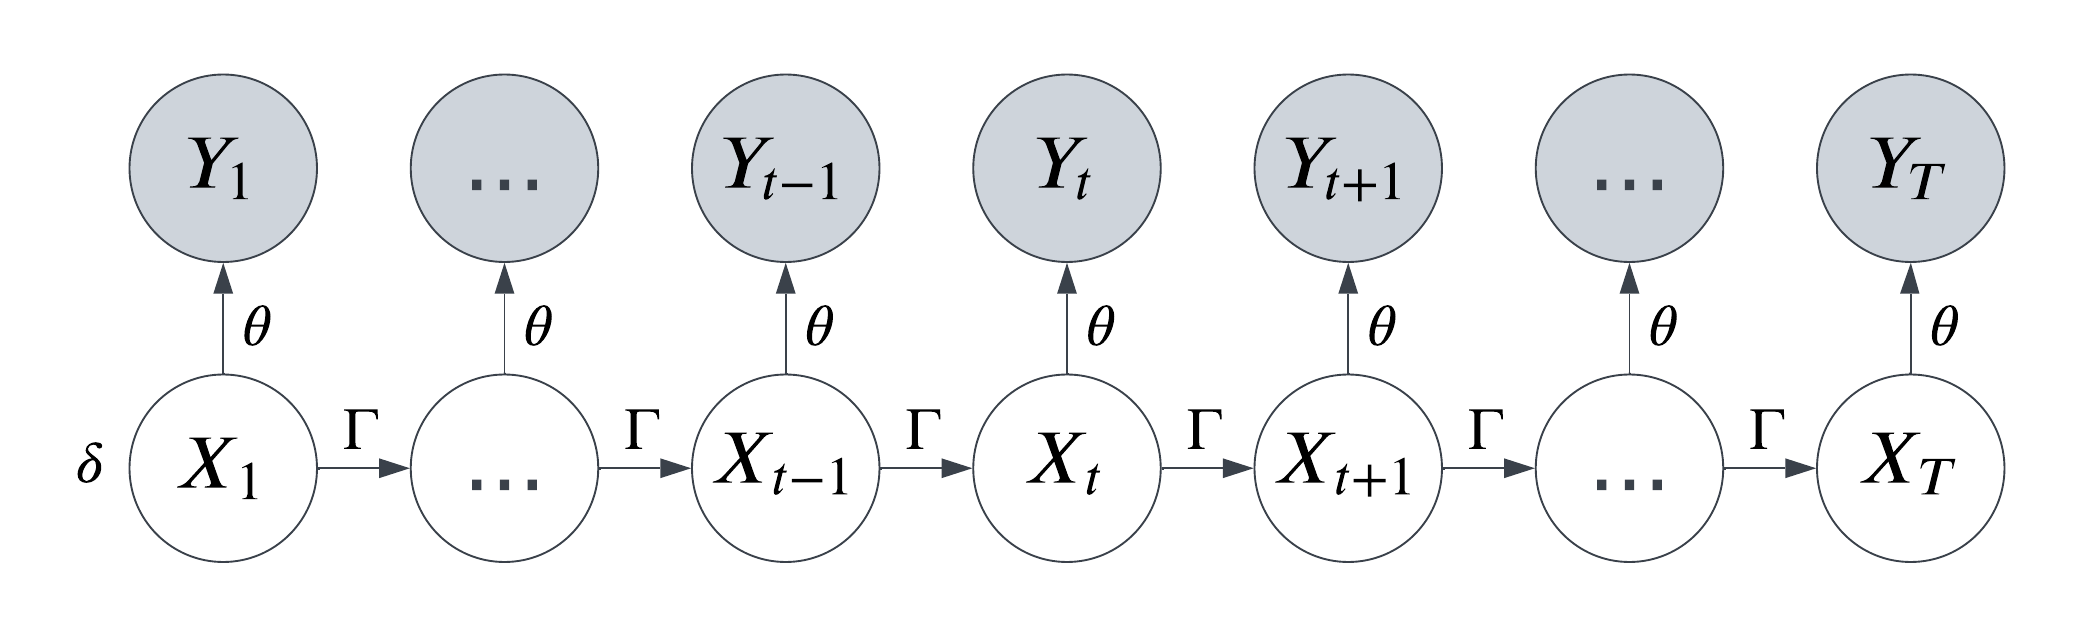
\includegraphics[width=5in]{../plt/HMM.png}
    \caption{Graphical representation of an HMM. $X_t$ corresponds to an unobserved latent state at time $t$ whose distribution is described by a Markov chain. $Y_t$ corresponds to an observation at time $t$, where $Y_t$ given all other observations $\bfY \setminus \{Y_t\}$ and hidden states $\bfX$ depends only on $X_t$.}
    \label{fig:HMM}
\end{figure}

It is convenient to reparameterize the transition probability matrix $\Gamma \in \bbR^{N \times N}$ and initial distribution $\delta \in \bbR^N$ in terms of an auxiliary variable $\eta$ to ensure that all entries are positive and all rows sum to one. One natural option is to use a softmax parameterization: %follow the parameterization of \citet{Barajas:2017}:
%
\begin{equation}
    \Gamma^{(i,j)}(\eta) = \frac{\exp(\eta^{(i,j)})}{\sum_{k=1}^N \exp(\eta^{(i,k)})}, \qquad \delta^{(i)}(\eta) = \frac{\exp(\eta^{(i)})}{\sum_{k=1}^N \exp(\eta^{(k)})}
    \label{eqn:reparam}
\end{equation}
%
where $i,j = 1,\ldots,N$ and $\eta^{(i,i)}$ and $\eta^{(1)}$ are set to zero for identifiability. This formulation simplifies likelihood maximization by removing constraints in the optimization problem. One may also incorporate covariates into $\Gamma$ by setting $\eta_t^{(i,j)}(\beta) = \left(\beta^{(i,j)}\right)^T \bfz_t$, where $\bfz_t$ is a column vector of known covariates at time index $t$ and $\beta^{(i,j)}$ is a column vector of unknown regression coefficients. While $\Gamma$ and $\delta$ are functions of $\eta$, we abuse notation in future sections and treat $\Gamma$ and $\delta$ as variables since the mapping is a bijection.
%
For brevity, we denote $\phi \equiv \{\theta,\eta\}$, $\eta^{(\cdot)} = \{\eta^{(i)}\}_{i=1}^N$, 
$\eta^{(i,\cdot)} = \{\eta^{(i,j)}\}_{j=1}^N$, and $\eta^{(\cdot,\cdot)} = \{\eta^{(i,j)}\}_{i,j=1}^N$. 

The joint likelihood of an HMM given observations $\bfY$ and latent states $\bfX$ is
%
\begin{equation}
    p(\bfX,\bfY;\phi) = \delta^{(X_1)} f^{(X_1)}(Y_1; \theta^{(X_1)}) \prod_{t=2}^T \Gamma^{(X_{t-1},X_t)} f^{(X_t)}(Y_t; \theta^{(X_t)}).
    \label{eqn:like}
\end{equation}
%
Alternatively, the marginal likelihood of the observed data $\bfY$ alone is 
%
\begin{equation}
    p(\bfY;\phi) = \delta P(Y_1;\theta) \prod_{t=2}^T \Gamma P(Y_t;\theta) \mathbf{1}_N.
    \label{eqn:like_marginal}
\end{equation}
%
where $\mathbf{1}_N$ is an $N$-dimensional column vector of ones and $P(y_t;\theta)$ is an $N \times N$ diagonal matrix with the $(i,i)^{th}$ entry $f^{(i)}(y_t; \theta^{(i)})$. For a more complete introduction to HMMs, see \citet{Zucchini:2016}.


\subsection{Variations of Hidden Markov Models}
\label{subsec:HHMM}

Hidden Markov models rely on several assumptions that are often violated in real-world applications. For example, high-frequency data often violates the assumption that the underlying state process of an HMM is time-homogeneous %, and that the observations are independent when conditioned on the hidden state process 
\citep{Sidrow:2021}. As such, researchers have introduced several variations, such as incorporating covariates into the transition probability matrix $\Gamma$ to account for changing dynamics in the transition matrix \citep{McClintock:2018}. In addition, if a sequence of observations displays multi-scale dependence structure, then it may be more appropriate to use a \textit{hierarchical} hidden Markov model, or HHMM \citep{Barajas:2017,Adam:2019,Sidrow:2021}. Hierarchical HMMs are useful because they capture dependence structures of the hidden process on multiple time scales. There are many different particular ways to define a Hierarchical HMM, such as the formulations in \citet{Barajas:2017}, \citet{Adam:2019}, and \citet{Sidrow:2021}. As presented here, Hierarchical HMMs involve some coarse-scale hidden process that evolves over time. While the coarse-scale state remains in the same state, a fine-scale hidden process evolves simultaneously. Observations are then generated according to a distribution that depends jointly on both the hidden coarse-scale state and the hidden fine-scale state. However, once the coarse-scale process changes states, the fine-scale process restarts and evolves depending upon that new coarse-scale state.

The parameters of an HHMM are defined to enforce this hierarchical structure for the hidden Markov chain. In particular, define a coarse-scale Markov chain $\{X^{(c)}_t\}_{t=1}^T$ parameterized by a pre-determined number of coarse-scale hidden states $N^{(c)} \in \bbN$, a coarse-scale initial distribution $\delta^{(c)} \in \bbR^{N^{(c)}}$ and coarse-scale probability transition matrix $\boldsymbol{\Gamma}^{(c)} \in \bbR^{{N^{(c)}} \times {N^{(c)}}}$. For each coarse-scale state $i$, we yet define another fine-scale Markov chain with states $X^{(f)}_t$ whose length is randomly determined by the dwell time of the coarse-scale Markov chain in state $i$. The $i^{th}$ fine-scale Markov chain is parameterized by a pre-determined number of fine-scale states $N^{(f,i)} \in \bbN$. It also has initial distribution $\delta^{(f,i)} \in \bbR^{N^{(f,i)}}$, and a fine-scale transition probability matrix $\boldsymbol{\Gamma}^{(f,i)} \in \bbR^{N^{(f,i)} \times N^{(f,i)}}$. In summary, 
%
\begin{gather}
    \delta^{(c,i)} = \bbP\left( X_1^{(c)} = i \right) \qquad 
    \Gamma^{(c,i,j)} = \bbP\left( X_{t+1}^{(c)} = j | X_{t}^{(c)} = i \right) \\
    %
    \delta^{(f,i,i')} = \bbP\left( X_{t+1}^{(f)} = i' | X_{t}^{(c)} \neq i, X_{t+1}^{(c)} = i \right) \qquad 
    \Gamma^{(f,i,i',j')} = \bbP\left( X_{t+1}^{(f)} = j' | X_{t}^{(f)} = i', X_{t}^{(c)} = i, X_{t+1}^{(c)} = i \right).
\end{gather}
%
Define the matrix $\boldsymbol{\Pi}^{(f,i)}$ as an $N^{(f,i)} \times N^{(f,i)}$ matrix with identical row entries $\delta^{(f,i)}$. Using this parameterization, the set of pairs $\{(X^{(c)}_t,X^{(f)}_t)\}_{t=1}^T$ is itself Markov chain. It has a total of $N \equiv \sum_{i=1}^{N^{(c)}} N^{(f,i)}$ hidden states, a global initial distribution of
%
\begin{equation} 
\boldsymbol{\delta} = 
\begin{pmatrix}
\delta^{(c,1)}\boldsymbol{\delta}^{(f,1)} & \delta^{(c,2)}\boldsymbol{\delta}^{(f,2)}    & \cdots & \delta^{(c,N^{(c)})}\boldsymbol{\delta}^{(f,N^{(c)})}
\end{pmatrix},
\label{eqn:global_delta}
\end{equation}
%
and a global probability transition matrix of %\textcolor{red}{I stole this from Vianey}:
%
\begin{equation} 
\boldsymbol{\Gamma} = 
\begin{pmatrix}
\Gamma^{(c,1,1)}\boldsymbol{\Gamma}^{(f,1)}     & \Gamma^{(c,1,2)} \boldsymbol{\Pi}^{(f,2)}     & \cdots & \Gamma^{(c,1,N^{(c)})}\boldsymbol{\Pi}^{(f,N^{(c)})}  \cr
\Gamma^{(c,2,1)}\boldsymbol{\Pi}^{(f,1)} & \Gamma^{(c,2,2)} \boldsymbol{\Gamma}^{(f,2)}  & \cdots & \Gamma^{(c,2,N^{(c)})}\boldsymbol{\Pi}^{(f,N^{(c)})} \cr
\vdots & \vdots & \ddots & \vdots \cr 
\Gamma^{(c,N^{(c)},1)}\boldsymbol{\Pi}^{(f,1)} & \Gamma^{(c,N^{(c)},2)}\boldsymbol{\Pi}^{(f,2)}      & \cdots & \Gamma^{(c,N^{(c)},N^{(c)})} \boldsymbol{\Gamma}^{(f,N^{(c)})} 
\end{pmatrix}.
\label{exptpm2}
\end{equation}
%
%corresponds to the probability that the initial coarse-scale hidden state is $i$, and $\Gamma^{(c,i,j)}$ corresponds to the probability that the coarse-scale hidden state will transition to coarse-scale state $j$ given that the current coarse-scale state is $i$. Further, $\delta^{(f,i,i')}$ corresponds to the probability that the initial fine-scale hidden state is $i'$ after transitioning to state $i$ from another state. Finally, $\Gamma^{(f,i,i',j')}$ corresponds to the probability that the fine-scale hidden state will transition to state $j'$ given that the current coarse-scale state is $i$ and the current fine-scale state is $i'$.
%
%Namely, $\delta^{(c,i)} = \bbP\left(X_1^{(c)}\right)$ corresponds to the probability that the initial coarse-scale hidden state is $i$, and $\Gamma^{(c,i,j)}$ corresponds to the probability that the coarse-scale hidden state will transition to coarse-scale state $j$ given that the current coarse-scale state is $i$. Further, $\delta^{(f,i,i')}$ corresponds to the probability that the initial fine-scale hidden state is $i'$ after transitioning to state $i$ from another state. Finally, $\Gamma^{(f,i,i',j')}$ corresponds to the probability that the fine-scale hidden state will transition to state $j'$ given that the current coarse-scale state is $i$ and the current fine-scale state is $i'$.
%
The transition probability matrix $\boldsymbol{\Gamma}$ and initial distribution $\boldsymbol{\delta}$ of a hierarchical HMM is simply a more restricted version of the same parameters for a standard HMM. A visualization of a hierarchical Markov chain with $N^{(c)} = 2$ and $N^{(f,1)} = N^{(f,2)} = 2$ is shown in Figure (\ref{fig:HHMM}).
%
\begin{figure}
    \centering
    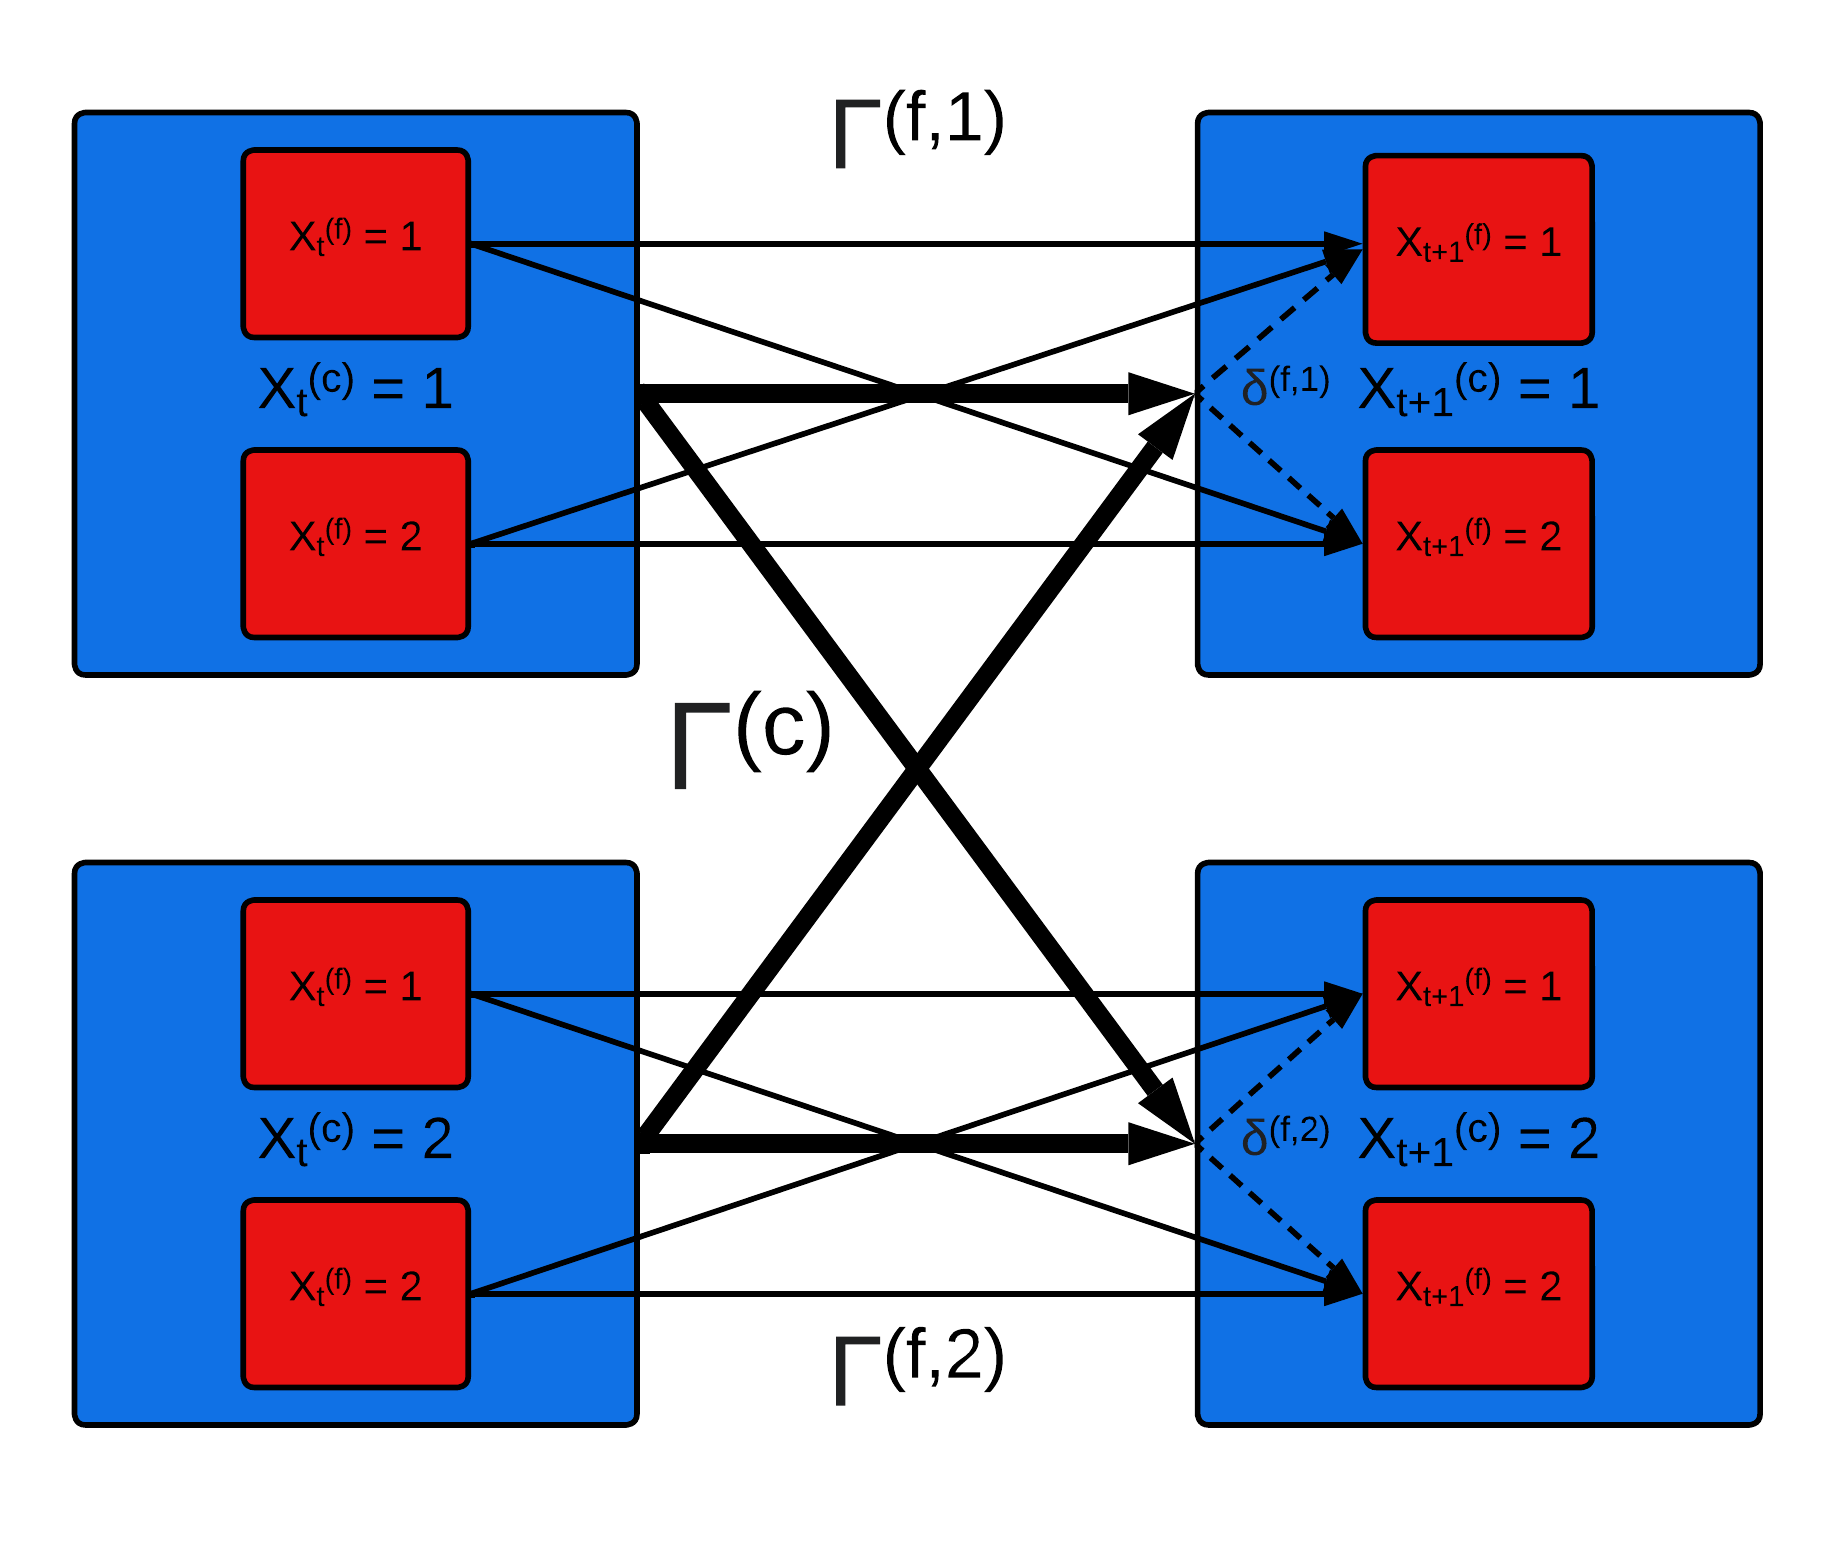
\includegraphics{plt/HHMM.png}
    \caption{Visualization of the underlying Markov chain for a hierarchical HMM with $N^{(c)} = 2$ and $N^{(f,1)} = N^{(f,2)} = 2$. Solid thick lines correspond to entries of $\boldsymbol{\Gamma}^{(c)}$. Solid thin lines correspond to entries of $\boldsymbol{\Gamma}^{(f,i)}$ for $i = 1,2$, which describes the distribution of $X_{t+1}^{(f)}$ if $X^{(c)}_{t} = X^{(c)}_{t+1} = i$. Dashed thin lines correspond to entries of $\boldsymbol{\delta}^{(f,i)}$ for $i = 1,2$, which describes the distribution of $X_{t+1}^{(f)}$ if $X^{(c)}_{t} \neq X^{(c)}_{t+1} = i$.}
    \label{fig:HHMM}
\end{figure}

The coarse-scale and fine-scale initial distributions and transition probability matrices are parameterized similarly to Equation (\ref{eqn:reparam}). In particular, $\boldsymbol{\Gamma}^{(c)}$ and $\boldsymbol{\delta}^{(c)}$ are parameterized via $\eta^{(c)}$ as follows:
%
\begin{equation}
    \Gamma^{(c,i,j)}(\eta^{(c)}) = \frac{\exp(\eta^{(c,i,j)})}{\sum_{k=1}^N \exp(\eta^{(c,i,k)})}, \qquad \delta^{(c,i)}(\eta^{(c)}) = \frac{\exp(\eta^{(c,i)})}{\sum_{k=1}^N \exp(\eta^{(c,k)})}
    \label{eqn:reparam_coarse}
\end{equation}
%
Likewise, $\boldsymbol{\Gamma}^{(f,i)}$ and $\delta^{(f,i)}$ are parameterized via $\eta^f$ as follows:
%
\begin{equation}
    \Gamma^{(f,i,i',j')}(\eta^f) = \frac{\exp(\eta^{(f,i,i',j')})}{\sum_{k'=1}^N \exp(\eta^{(f,i,i',k')})}, \qquad \delta^{(f,i,i')}(\eta^{f}) = \frac{\exp(\eta^{(f,i,i')})}{\sum_{k'=1}^N \exp(\eta^{(f,i,k')})}.
    \label{eqn:reparam_fine}
\end{equation}
%
%Finding closed-form solutions to the M-step for an HHMM is not straightforward, so it may be preferable to use numerical maximization techniques. We therefore review different methods for numerical maximization via stochastic optimization.


\subsection{State Decoding}

One appealing feature of HMMs is that it is simple to determine the probability distribution of the hidden state at time $t$, $X_t$, conditional of the set of observations $Y_t$. Define the probability density of the observations between times $s$ and $t$ as $p(y_{s:t};\phi)$. Likewise, define \textit{forward probabilities} $\alpha^{(i)}_t = p(y_{1:t},X_t = i;\phi)$ (for $i = 1,\ldots,N$ and $t = 1,\ldots,T$) and \textit{backward probabilities} $\beta^{(i)}_t = p(y_{(t+1):T}|X_t = i;\phi)$ (for $i = 1,\ldots,N$ and $t = 1,\ldots,T-1$). By convention, $\beta^{(i)}_T = 1$ for $i = 1,\ldots,N$. 
Both $\alpha_t$ and $\beta_t$ can be defined recursively:
%
\begin{align}
    \alpha_1^{(i)}(\phi) &= \delta^{(i)} f^{(i)}(y_1;\theta^{(i)}), & \alpha_t^{(i)}(\phi) &= \sum_{j=1}^N \alpha_{t-1}^{(j)} \Gamma^{(j,i)} f^{(i)}(y_t;\theta^{(i)}), \quad t = 2,\ldots,T. \label{eqn:alpha} \\
    %
    \beta_T^{(i)}(\phi) &= 1, & \beta_t^{(i)}(\phi) &= \sum_{j=1}^N \Gamma^{(i,j)} f^{(j)}(y_{t+1};\theta) \beta^{(j)}_{t+1}, \quad t = 1,\ldots,T-1. \label{eqn:beta}
\end{align}

We denote the probability that $X_t = i$ given all observations $\bfY$ and parameters $\phi$ as $\gamma_t^{(i)}(\phi)$ for $t = 1,\ldots,T$ and $i = 1,\ldots,N$. Further, we denote the probability that $X_{t-1} = i$ and $X_t = j$ given all observations $\bfY$ and parameters $\phi$ as $\xi_t^{(i,j)}(\phi)$ for $t = 2,\ldots,T$ and $i,j = 1,\ldots,N$. Namely,
%
\begin{gather}
    \gamma_t^{(i)}(\phi) = \bbP(X_t = i \mid \bfY ~;~ \phi), \\ \xi_t^{(i,j)}(\phi) = \bbP(X_{t-1} = i, X_t = j \mid \bfY ~;~ \phi). \nonumber
\end{gather}
%
Both $\gamma_t$ and $\xi_t$ can be calculated from $\alpha_{t-1}$, $\alpha_t$, and $\beta_t$:
%
\begin{gather}
    \gamma_{t}^{(i)}(\phi) = \frac{\alpha_{t}^{(i)} ~ \beta_{t}^{(i)}}{\sum_{i'} \alpha_{t}^{(i')} ~ \beta_{t}^{(i')}}, \label{eqn:gamma} \\
    %
    \xi_{t}^{(i,j)}(\phi) = \frac{\alpha_{t-1}^{(i)} ~ \Gamma^{(i,j)} ~ f^{(j)}(y_{t} ~ ; ~\theta) ~ \beta_{t}^{(j)}}{\sum_{i',j'} ~ \alpha_{t-1}^{(i')} ~ \Gamma^{(i',j')} ~ f^{(j')}(y_{t} ~ ; ~\theta) ~ \beta_{t}^{(j')}} \label{eqn:xi},
\end{gather}

\subsection{The Baum-Welch Algorithm}

The Baum-Welch algorithm is a specific instance of the EM algorithm used to estimate the parameters of the HMM. Suppose a sequence of observations $\bfY$ is observed as output of an latent-variable model with unknown latent states $\bfX$ and unknown parameters $\phi$. At iteration $k$ of the EM algorithm, denote the current parameter estimates as $\phi_{k}$. One iteration of the EM algorithm consists of and expectation (or E) step, followed by a maximization (or M) step. For the E step, the function $Q(\phi \mid \phi_{k})$ is defined as the expected value of the joint log-likelihood $\log p(\bfY,\bfX; \phi)$ when $\bfX$ is a random variable with density $p(\bfX | \bfY ; \phi_{k})$. For the M step, the next parameter estimate $\phi^{k+1}$ is found by maximizing $Q(\phi \mid \phi_{k})$ with respect to the parameters $\phi$:
%
\begin{gather}
    Q(\phi \mid \phi_{k}) \equiv \bbE_{\phi_{k}}\left[\log p(\bfY,\bfX;\phi) \mid \bfY \right] \label{eqn:Q} \\
    %
    %Q^*(\phi_{k}) \equiv \max_{\phi}Q(\phi \mid \phi_{k})\\
    %
    \phi_{k+1} = \argmax_{\phi} Q(\phi \mid \phi_{k}). \label{eqn:BW_update}
\end{gather}
%
When the EM algorithm is applied to HMMs, it is called the \textit{Baum-Welch} algorithm. We can combine Equation (\ref{eqn:Q}) with Equation (\ref{eqn:like}) to separate the expected value into three convenient terms:
\begin{align}
    Q(\phi \mid \phi_{k}) &\equiv \bbE_{\phi_{k}}\left[\log p(\bfY,\bfX;\phi) \mid \bfY \right] \\
    &= \bbE_{\phi_{k}} \left[\sum_{t=1}^T \log f^{(X_t)}(y_t;\theta^{(X_t)}) + \log \delta^{(X_1)} + \sum_{t=2}^{T} \log \Gamma^{(X_{t-1},X_{t})} \mid \bfY \right] \\
    %
    &= \sum_{t = 1}^T \bbE_{\phi_{k}} \left[ \log f^{(X_t)}(y_t;\theta^{(X_t)}) \mid \bfY \right]  \\
    & \qquad + \bbE_{\phi_{k}} \Big[\log \delta_{X_1} \mid \bfY \Big] + \sum_{t=2}^{T} \bbE_{\phi_{k}} \left[ \log \Gamma^{(X_{t-1},X_{t})} \mid \bfY \right] \\
    %
    &= \sum_{t = 1}^T \sum_{i=1}^N \gamma^{(i)}_t(\phi_{k}) \log f^{(i)}(y_t;\theta^{(i)}) \\
    & \qquad + \sum_{i=1}^N \gamma^{(i)}_1(\phi_{k}) \log \delta^{(i)} + \sum_{t=2}^{T} \sum_{i=1}^N \sum_{j=1}^N \xi_t^{(i,j)}(\phi_{k}) \log \Gamma^{(i,j)}.
\end{align}

The first term and last two terms on the right-hand side of the equation above only depend upon $\theta$ and $\eta$, respectively. The maximization problem in Equation (\ref{eqn:BW_update}) can thus be divided into two separate sub-problems as follows. Note that we define the objective functions $F$ and $G$ below so that the M-step of the EM algorithm is a minimization problem consistent with existing optimization literature.
%
\begin{gather}
    F_t^{(k)}(\theta) \equiv F_t(\theta, \phi_{k}) \equiv - \sum_{i=1}^N \gamma^{(i)}_t(\phi_{k}) \log f^{(i)}(y_t;\theta^{(i)}), \\
    %
    F^{(k)}(\theta) \equiv F(\theta, \phi_{k}) \equiv \frac{1}{T} \sum_{t=1}^T F^{(k)}_t(\theta), \label{eqn:F} \\
    %
    \theta_{k+1} = \argmin_{\theta} F^{(k)}(\theta), \label{eqn:EM_update_theta} \\ \nonumber \\
    %
    %
    G_1^{(k)}(\eta) \equiv G_1(\eta, \phi_{k}) \equiv - \sum_{i=1}^N \gamma^{(i)}_1(\phi_{k}) \log \delta^{(i)}(\eta) \\
    %
    G_t^{(k)}(\eta) \equiv G_t(\eta, \phi_{k}) \equiv - \sum_{i=1}^N \sum_{j=1}^N \xi^{(i,j)}_t(\phi_{k}) \log \Gamma^{(i,j)}(\eta), \quad t \geq 2 \\
    %
    G^{(k)}(\eta) \equiv G(\eta, \phi_{k}) = \frac{1}{T} \sum_{t=1}^{T} G_t(\eta, \phi_{k}), \label{eqn:G}\\
    %
    \eta_{k+1} = \argmin_{\eta} G(\eta,\phi_{k}). \label{eqn:EM_update_eta}
\end{gather}
In addition, note that 
\begin{equation}
   Q(\phi \mid \phi_{k}) = -T ~ \left[F(\theta, \phi_{k}) + G(\eta, \phi_{k})\right].
\end{equation}
%
In many simple scenarios the maximization problems above have closed-form solutions. For example, if $\Gamma$ does not depend upon any covariates and $f^{(i)}(y_t;\theta^{(i)})$ is a normal or Poisson probability density function with respect to $y_t$, then the solutions of Equations (\ref{eqn:EM_update_theta}) and (\ref{eqn:EM_update_eta}) are given in Section 4.2 of \citet{Zucchini:2016}. However, in many other situations, the maximization problem above is not straightforward and requires numerical maximization techniques. For example, finding closed-form solutions to the M-step for the HHMM defined in section \ref{subsec:HHMM} is not straightforward. We therefore review different methods for numerical maximization via stochastic optimization. %We describe several such scenarios in the subsequent section. 

\subsection{Stochastic Optimization}
\label{subsec:stoch_optim}

Stochastic optimization techniques can solve minimization problems that can be written as the sum of independent terms, including the one posed in Equation (\ref{eqn:EM_update_theta}) to optimize $\theta$ at step $k$ in the EM algorithm \citep{Robbins:1951}.
%
\begin{equation}
    \theta_{k+1} = \argmin_{\theta} F^{(k)}(\theta), \qquad F^{(k)}(\theta) = \frac{1}{T}\sum_{t = 1}^T F^{(k)}_t(\theta).
\end{equation}
%
Similar logic can be applied to optimizing $\eta$ in Equation (\ref{eqn:EM_update_eta}).
%
Standard gradient descent updates $\theta_k$ using an iterative process. Note that $k$ indexes the iteration of the EM algorithm, as we use $m$ to index the iteration of gradient descent within the $k^{th}$ M-step the EM algorithm. As such, gradient descent at step $m$ has the following update rule with step size $\lambda_F$:
%
\begin{equation}
    \theta_{k,m+1} = \theta_{k,m} - \lambda_F \nabla F^{(k)}(\theta_{k,m}) =  \theta_{k,m} - \frac{\lambda_F}{T} \sum_{t=1}^T \nabla F^{(k)}_t(\theta_{k,m}).
\end{equation}
%
However, this update requires evaluating a gradient for all $t = 1,\ldots,T$, which can be prohibitive if $T$ is large. Alternatively, \citet{Robbins:1951} introduce stochastic gradient descent (or SGD), which updates $\theta_k$ using an unbiased estimate of the full gradient:
%
\begin{equation}
    \theta_{k,m+1} = \theta_{k,m} - \lambda_F \nabla F^{(k)}_{t_{k,m}}(\theta_{k,m})
\end{equation}
%
for some $t_{k,m} \in \{1,\ldots,T\}$ selected uniformly at random at step $m$ of M-step $k$. Stochastic gradient descent reduces the amount of time between updates by using an unbiased estimate of the gradient to update $\theta_{k,m}$. However, the gradient estimates themselves can have high variance, so stochastic gradient descent requires that the step-size $\lambda_F$ decays over time to ensure convergence. In addition, SGD has slower convergence rates compared to full gradient descent \citep{Schmidt:2017}.

Variance-reduced stochastic optimization techniques such as stochastic average gradient descent (SAG) \citep{Schmidt:2017}, stochastic variance reduced gradient descent (SVRG) \citep{Johnson:2013}, and SAGA \citep{Defazio:2014} enjoy the speed of stochastic gradient descent as well as the convergence rates of full gradient descent. These algorithms involve a table of gradient estimates $\widehat \nabla F^{(k)}_t$ whose average approximates the full gradient $\nabla F^{(k)}(\theta_{k,m})$. The gradient estimates are updated at various stages in the optimization algorithm and are used to reduce the variance of gradient estimates. 
%In particular, SAG uses the update rule:
%
%\begin{equation}
%    \theta_{m+1} \gets \theta_{m} - \lambda_F \left[\frac{\nabla F^{(k)}_{t_m}(\theta_{m}) - \widehat \nabla F^{(k)}_{t_m}}{T} + \frac{1}{T} \sum_{t=1}^T \widehat \nabla F^{(k)}_{t} \right], \label{eqn:SAG_update}
%\end{equation}
%
%which is simply the table average with entry $t_m$ updated at step $m$. This update rule is intuitive, but it represents a biased estimate of the gradient $\nabla P(\theta_m)$. This can slow down convergence and makes theoretical analysis of SAG difficult. 
For example, SVRG and SAGA update $\theta_{k,m}$ using an unbiased estimate of the gradient:
%
\begin{equation}
    \theta_{k,m+1} = \theta_{k,m} - \lambda_F \left[\nabla F^{(k)}_{t_{k,m}}(\theta_{k,m}) - \widehat \nabla F^{(k)}_{t_{k,m}} + \widehat \nabla F^{(k)} \right],
    \label{eqn:SAGA_update}
\end{equation}
%
where:
%
\begin{equation}
    \widehat \nabla F^{(k)} = \frac{1}{T} \sum_{t=1}^T \widehat \nabla F^{(k)}_{t}.
    \label{eqn:tbl_avg}
\end{equation}
%Taking the expected value of the gradient estimate from (\ref{eqn:SAGA_update}) shows that it is unbiased:
%
%\begin{align}
%    \bbE\left[\nabla F^{(k)}_{t_m}(\theta_{m}) - \widehat \nabla F^{(k)}_{t_m} + \frac{1}{T} \sum_{t=1}^T \widehat \nabla F^{(k)}_{t} \right] &= \frac{1}{T} \sum_{t=1}^T \nabla F^{(k)}_{t}(\theta_{m}) - \frac{1}{T} \sum_{t=1}^T \widehat \nabla F^{(k)}_{t} + \frac{1}{T} \sum_{t=1}^T \widehat \nabla F^{(k)}_{t} \\
    %
%    &= \frac{1}{T} \sum_{t=1}^T \nabla F^{(k)}_{t_m}(\theta_{m}) = \nabla F^{(k)}(\theta_{m}).
%\end{align}
%
After updating the parameters at step $m$ of iteration $k$, SAGA simply updates the table average and the table of gradients at position $t_{k,m}$: 
%
\begin{gather}
    \widehat \nabla F^{(k)} \gets \widehat \nabla F^{(k)} + \nabla F^{(k)}_{t_{k,m}}(\theta_{k,m}) - \widehat \nabla F^{(k)}_{t_{k,m}}, \\
    %
    \widehat \nabla F^{(k)}_{t_{k,m}} \gets \nabla F^{(k)}_{t_{k,m}}(\theta_{k,m}).
\end{gather}
%
%After updating the table at position $t_m$ with the SAG/SAGA update rule, the table average $\frac{1}{T} \sum_{t=1}^T \widehat \nabla F^{(k)}_{t}$ must be updated using the previous estimate of $\widehat \nabla F^{(k)}_{t}$. 

Traditionally, SAGA is more memory intensive than SVRG because the gradient at every index must be stored. However, the Baum-Welch algorithm involves storing weights for each time index $t$ to define the $Q-$ function, so storing each gradient for SAGA is not any more memory intensive than the Baum-Welch algorithm itself. Alternatively, SVRG is more computationally intensive than SAGA partially because it requires the table average $\widehat \nabla F$ to be occasionally refreshed, which involves a full pass of the data set. However, the E-step of the Baum-Welch algorithm involves a full pass of the data set, using SVRG is not any more computationally expensive than the Baum-Welch algorithm itself. Therefore, using either algorithm in the M-step of the Baum-Welch algorithm adds minimal computational and memory complexity.

%This trade-off should be considered by practitioners when deciding between the two algorithms. 

Algorithm (\ref{alg:SO}) outlines SVRG and SAGA in pseudocode.

\begin{algorithm}
\caption{Summary of SVRG and SAGA}\label{alg:SO}
\begin{algorithmic}[1]
\Require Loss function $P = \sum_t P_t$, Initial value $z_0$, step size $\lambda$, algorithm (SVRG or SAGA), number of full gradient updates $K$ (classically, $K = 1$ for SAGA), and iterations per full gradient update $M$.
%
\For{$k = 0,\ldots,K-1$}
\State Initialize gradient estimates $\widehat \nabla P_t \leftarrow \nabla P_t (z_k)$ for $t = 1, ..., T$ and table average $ \widehat \nabla P \gets \frac{1}{T} \sum_{t=1}^T \widehat \nabla P_{t}.$
\State Initialize $z_{k,0} \leftarrow z_k$.
%
\For{$m = 0,1,\ldots,M-1$}:
    %
    \State Pick $t_{k,m} \in \{1,\ldots,T\}$ uniformly at random.
    %
    \State \Comment{update parameters}
    \begin{equation}
        z_{k,m+1} = z_{k,m} - \lambda \left[\nabla P_{t_{k,m}}(z_{k,m}) - \widehat \nabla P_{t_{k,m}} + \widehat \nabla P \right]
        \label{eqn:SAGA_update0}
    \end{equation}
    %
    \If{using SAGA}:
    \Comment{update table average and table at index $t_{k,m}$}
        \begin{gather}
            \widehat \nabla P \gets \widehat \nabla P + \nabla P_{t_{k,m}}(z_{k,m}) - \widehat \nabla P_{t_{k,m}}, \\
            \widehat \nabla P_{t_{k,m}} \leftarrow \nabla P_{t_{k,m}}(z_{k,m}).
        \end{gather}
    \EndIf
\EndFor
\State $z_{k+1} = z_{k,M}$
\EndFor
\State \Return $z_K$
\end{algorithmic}
\end{algorithm}


%Whether or not Equations (\ref{eqn:EM_update_theta}) and (\ref{eqn:EM_update_eta}) have closed-form solutions, even defining $F^{(k)}$ and $G^{(k)}$ to initialize the optimization problem (the E-step) has a time cost of $\calO(T)$, which can be expensive for large $T$. 


%%%%%%%%%%%%



\iffalse
\subsection{Direct likelihood maximization}

An alternative way to perform inference over HMMs is to directly maximize the marginal likelihood from Equation (\ref{eqn:like_marginal}) using gradient-based optimization techniques. One standard method is gradient descent, which updates $\theta$ or $\eta$ at step $m$ using the following update rule with step sizes $\lambda_F^\eta$ and $\lambda_F^\theta$:
%
\begin{gather}
    \eta_{m+1} = \eta_{m} + \lambda_F^{\eta} \nabla_\eta \log p(\bfY;\theta_{m},\eta_{m}) \\
    %
    \theta_{m+1} = \theta_{m} + \lambda_F^{\theta} \nabla_\theta \log p(\bfY;\theta_{m},\eta_{m}).
    \label{eqn:grad_update}
\end{gather}
%
Using the Fisher identity of the gradient for incomplete data models \citep{Fisher:1925}, the gradient of Equation (\ref{eqn:like_marginal}) can be written as
%
\begin{equation}
    \nabla_{\phi} \log p(\bfY;\phi) = \bbE_{\phi}\left[ \nabla_{\phi} \log p(\bfY,\bfX;\phi) \mid \bfY \right].
    \label{eqn:fisher_id}
\end{equation}
%
Similarly to the EM algorithm, we can split the gradient of the log-likelihood into separate terms that each depend on only $\theta$ or $\eta$:
%
\begin{gather}
    \nabla_{\theta} \log p(\bfY;\phi) = \sum_{t=1}^T \sum_{i=1}^N \gamma_t^{(i)}(\phi) \nabla_{\theta} \log f^{(i)}(y_t;\theta^{(i)}) \label{eqn:theta_update_gd} \\
    %
    \nabla_{\eta} \log p(\bfY;\phi) = \sum_{i=1}^N \gamma_1^{(i)}(\phi) \nabla_{\eta} \log \delta^{(i)} + \sum_{t=2}^{T} \sum_{i=1}^N \sum_{j=1}^N \xi_t^{(i,j)}(\phi) \nabla_{\eta} \log \Gamma^{(i,j)}, \label{eqn:eta_update_gd}
\end{gather}
%
There is a clear connection between the Baum-Welch update from Equation (\ref{eqn:BW_update}) and the gradient given by Equation (\ref{eqn:fisher_id}). In particular, one recovers gradient descent by performing one gradient step within the M-step of the Baum-Welch algorithm rather than solving the entire maximization problem. This connection leads to a natural question: if taking one gradient step within the M- step is equivalent to gradient descent, and solving the M- step entirely results in the Baum-Welch algorithm, then are there other ways to perform the M-step in the EM algorithm with desirable properties? To answer this question, we first review some stochastic optimization techniques.
\fi
